
\section{Objectives}
By the end of this laboratory experiment, students are expected to learn how to:

\begin{itemize}

\item build electrical equivalent circuits for basic logic gates used in digital systems, and 
  
\item test integrated circuits consisting of basic logic gates. 
   
\end{itemize}

\section{Parts}
\label{sec:partsEx12}
The following parts are required to conduct this laboratory experiment: %
%
\begin{enumerate}           
\item Breadboard
\item One $330~[\ohm]$ resistor
\item Agilent E3630A power supply
\item One  LED
\item One SN7404\footnote{See datasheet at \url{http://www.ti.com/lit/ds/symlink/sn54ls04-sp.pdf}} NOT Gate IC
\item One SN7408\footnote{See datasheet at \url{http://www.ti.com/lit/ds/symlink/sn74ls08.pdf}}   AND Gate IC
\item One SN7432N\footnote{See datasheet at \url{http://www.ti.com/lit/ds/symlink/sn54ls32.pdf}}  OR Gate IC
  
\item Two SPST switches 
\end{enumerate}


\section{Introduction}
\label{sec:introduction}
Let us consider the binary logic that operates with variables that take on two values, such as (\emph{TRUE, FALSE}), (\emph{YES, NO}), (\emph{ON, OFF}), $(1,0),$ and so forth. For convenience, we shall work with binary variables that take on values of $1$ or $0$ value. For example, if $A$ is a binary variable, then $A\in\{0,1\}.$ The three fundamental logic operations in digital systems are: %
%
\begin{enumerate}
\item \emph{AND},
  
\item \emph{OR}, and
  
\item \emph{NOT}.
\end{enumerate}
%
The basic digital devices that implement the \emph{AND}, \emph{OR}, and \emph{NOT} operations are called \emph{AND gate}, \emph{OR gate}, and \emph{NOT gate}, respectively. A brief description of each of these gates is given below.

\subsection{AND Gate}
\label{sec:andGate}
The AND gate is a two-input, one output digital device. Let us define $A$ and $B$ as binary variables representing the two inputs, and $L$ as a binary variable representing the output of the \emph{AND} gate.  Note that $A,~B,$ and $L$ take values from the set $\{0,1\},$~\textit{i.e.,}~$A,B,L\in\{0,1\}.$ The operation of the AND gate can easily be realized by an electrical circuit shown in Figure~\ref{fig:andGate}, where two SPST switches, $A$ and $B,$ represent inputs and the LED represents the output. The circuit has an input DC voltage,  $V_s,$ with a resistor $R$ connected in series to limit the current flowing through the LED. Note that $A=1(0)$ when the switch $A$ is closed (open). Similarly,   $B=1(0)$ when the switch $B$ is closed (open). The binary variable $L=1(0),$ when the LED is ON(OFF). Therefore, the output LED is ON if and only if both switches, $A$ and $B,$ are closed.  
%
\begin{figure}
  \centering
    \begin{circuitikz}[american voltages]
      \draw 
      (0,0)  to[V = $V_s$,invert,fill=green!50] (0,4*\smgrid) to [R,l=$R$](4*\smgrid,4*\smgrid) to[spst,l=A](7*\smgrid,4*\smgrid)to[spst,l=B](10*\smgrid,4*\smgrid) to[full led,l=~~LED (L)](10*\smgrid,0) to[short,-*](0,0)node[ground]{};
    \end{circuitikz}
  \caption{Electical circuit for implementing AND gate operations.}
  \label{fig:andGate}
\end{figure}
%
The operation of the circuit  is described by the \emph{truth table} shown in Table~\ref{tab:andGate}. %
%
\begin{table}
  \centering
  \caption{AND gate truth table.}
  \label{tab:andGate}  
  \begin{tabular}{l|l|l}
    \toprule
    A&B& $L= A~\mathrm{AND}~B$\\
    \toprule
    0 (OFF) & 0 (OFF) & 0 (OFF)\\
    0 (OFF) & 1 (ON) & 0 (OFF)\\
    1 (ON) & 0 (OFF) & 0 (OFF)\\
    1 (ON) & 1 (ON) & 1 (ON)\\
    \bottomrule
  \end{tabular}
\end{table}
%
The operation of the AND gate is expressed using a logic expression: $ L = A~\text{AND}~B,$ or $ L = A\cdot B,$ or simply $L = AB.$ For clarity, the logic expression for the  AND gate is mostly given by: %
%
\begin{align*}
 L= AB. 
\end{align*}
%
The logic symbol that represents the AND gate in digital systems is shown in Figure~\ref{fig:andGateSymbol}. %
%
\begin{figure}
  \centering
  \begin{circuitikz}
  \draw
   (0,0) node[american and port] (myAnd){}
   (myAnd.in 1) node[anchor = east]{A}
   (myAnd.in 2) node[anchor = east]{B}
   (myAnd.out) node[anchor = west]{L};
 \end{circuitikz}
 \caption{AND gate logic symbol.}
 \label{fig:andGateSymbol}
\end{figure}
%



\subsection{OR Gate}
\label{sec:orGate}
Similar to the AND gate digital device, the OR gate has two inputs and one output. The OR gate operation can be realized by the  electrical circuit shown in Figure~\ref{fig:orGate}, where two SPST switches, $A$ and $B,$ represent inputs and the LED represents the output. The output LED is ON when any of the switches is closed. 
%
\begin{figure}
  \centering
    \begin{circuitikz}[american voltages]
      \draw
      (0,0) to[V=$V_s$,invert,fill=green!50](0,4*\smgrid) to[R,l=$R$](4*\smgrid,4*\smgrid) -| (4*\smgrid,5*\smgrid) to[spst,l=A] (6*\smgrid,5*\smgrid) |-(8*\smgrid,4*\smgrid) to[full led, l=~~LED (L)] (8*\smgrid,0) to[short,-*](0,0)node[ground]{};
      \draw
      (4*\smgrid,4*\smgrid) -- (4*\smgrid,3*\smgrid) to[spst,l=B](6*\smgrid,3*\smgrid) --(6*\smgrid,4*\smgrid);
    \end{circuitikz}
  \caption{Electical circuit for implementing OR gate operations.}
  \label{fig:orGate}
\end{figure}
%


The operation of the OR gate circuit shown in Figure~\ref{fig:orGate} is summarized in the \emph{truth table} shown in Table~\ref{tab:orGate}. %
%
\begin{table}[H]
  \centering
  \caption{OR gate truth table.}
  \label{tab:orGate}  
  \begin{tabular}{l|l|l}
    \toprule
    A&B& $L= A~\mathrm{OR}~B$\\
    \toprule
    0 (OFF) & 0 (OFF) & 0 (OFF)\\
    0 (OFF) & 1 (ON) & 1 (ON)\\
    1 (ON) & 0 (OFF) & 1 (ON)\\
    1 (ON) & 1 (ON) & 1 (ON)\\
    \bottomrule
  \end{tabular}
\end{table}
%

The logic expression of the OR gate is: $ L = A~\text{OR}~B.$ However, it is usually expressed as: %
%
\begin{align*}
 L= A+B, 
\end{align*}
%
for convenience. Figure~\ref{fig:orGateSymbol} shows the symbol used to represent a logic OR gate. 
%
\begin{figure}
  \centering
  \begin{circuitikz}
    \draw
       (0,0) node[american or port] (myOr){}
       (myOr.in 1) node[anchor = east]{A}
       (myOr.in 2) node[anchor = east]{B}
       (myOr.out) node[anchor = west]{L};
 \end{circuitikz}
 \caption{OR gate logic symbol.}
 \label{fig:orGateSymbol}
\end{figure}
%

\subsection{NOT Gate}
\label{sec:notGate}
As opposed to AND and OR gates, the NOT gate has one input and one output. A logic circuit diagram that describes the operation of a NOT gate is shown in Figure~\ref{fig:notGate}. %
%
\begin{figure}[H]
  \centering
    \begin{circuitikz}[american voltages]
      \draw
      (0,0) to[V=$V_s$,invert,fill=green!50](0, 4*\smgrid);
      \draw
      (0,4*\smgrid) to[R,l=$R$](4*\smgrid,4*\smgrid) to[spst,l=A] (4*\smgrid,0)to[short,-*](0,0)node[ground]{};
      \draw
      (4*\smgrid,4*\smgrid) -- (8*\smgrid,4*\smgrid) to[full led, l=~~LED (L)] (8*\smgrid,0) -- (0,0); 
    \end{circuitikz}
%      
  \caption{Electical circuit for implementing NOT gate operations. }
  \label{fig:notGate}
\end{figure}
%
As can be seen from Figure~\ref{fig:notGate}, the LED is ON when the switch $A$ is open (OFF or logic $0$) and it is OFF when the switch $A$ is closed (ON or logic $1$). This operation is summarized in Table~\ref{tab:notGate}. %
%
\begin{table}[H]
  \centering
  \caption{NOT gate truth table.}
  \label{tab:notGate}  
  \begin{tabular}{l|l}
    \toprule
    A& $L= \mathrm{NOT}~A$\\
    \toprule
    0 (OFF) & 1 (ON)\\
    1 (ON) & 0 (OFF)\\
    \bottomrule
  \end{tabular}
\end{table}
%

The logic expression of the NOT gate is: $ L = \mathrm{NOT}~~A,$ or simply %
%
\begin{align*}
 L= A^{'}. 
\end{align*}
%
Figure~\ref{fig:notGateSymbol} shows the symbol used to represent a logic NOT gate. 
%
\begin{figure}[H]
  \centering
  \begin{circuitikz}
        \draw
       (0,0) node[american not port] (myNot){}
       (myNot.in) node[anchor = east]{A}
       (myNot.out) node[anchor = west]{L};
 \end{circuitikz}
 \caption{NOT gate logic symbol.}
 \label{fig:notGateSymbol}
\end{figure}
%

\subsection{Integrated Circuit}
\label{sec:IC}
A collection of digital devices (gates) fabricated into a single chip is called an integrated circuit (IC). Note that ICs can be categorized (depending on the number of gates fabricated into a single chip) as: %
\begin{itemize}
\item SSI (Small-scale integration): Integrated circuits contain $1$ to $20$ gates (SSI ICs),
\item MSI (medium scale integration): Integrated circuits contain $20$ to $200$ gates (MSI ICs),
\item LSI (large scale integration): Integrated circuits contain $200$ to $200,000$ gates (LSI ICs), and 
\item VLSI (very large scale integration): Integrated circuits contain over  $10^6$ transistors (as opposed to gates). 
\end{itemize}
%
Figure~\ref{fig:fig1-5} shows pin diagrams of a few SSI ICs, which are mostly used in building basic digital logic circuits. %
\begin{figure}
  \centering
  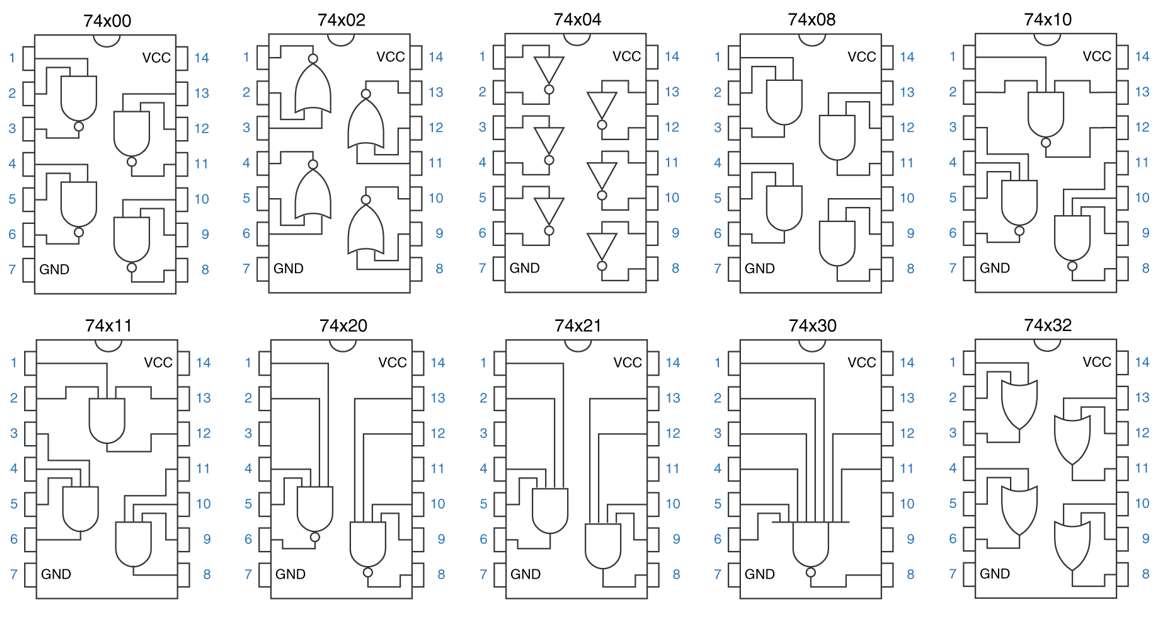
\includegraphics[width=0.7\textwidth]{figs/img/fig1-5}
  \caption{Pin diagram of a few 7400--series SSI ICs (image taken from~\cite{Wakerly2006})}
\label{fig:fig1-5}
\end{figure}
%
As can be seen, each 14-pin SSI IC has power supply $V_{\text{CC}}$ and \emph{GND} pins. An input is logic-1(0) when it is connected to $V_{\text{CC}}~(\text{GND}).$  
The SSI ICs 74x08, 74x32, and 74x04 contain four 2-input AND gates, four 2-input OR gates, and six NOT gates, respectively.    

\section{Prelab}
\label{sec:prelab}
It is important to read the previous section that details the basic digital devices used in building digital systems. Here, you will be working on simple logic expressions that make use of basic digital logic gates.  


\begin{prelab}[Logic circuit diagram]{prelab:logicCircuitDiagram}
  Consider the logic expression given by
  \begin{subequations}
  \label{eq:logicExpression}    
  \begin{align}
    \label{eq:F}
    F(A,B,C)&=C(A+B),\\
    \label{eq:G}
    G(A,B,C)&=\left[C(A+B)\right]^{'} = C^{'}+A^{'}B^{'},
  \end{align}    
  \end{subequations}
%
where $F$ and $G$ are the logic output functions of three binary variables $A,$ $B,$ and $C.$ Therefore, the binary variables $A,$ $B,$ $C,$ $F,$ and $G$ take values from the set $\{0,1\}.$
\begin{enumerate}
\item Determine number of inputs and outputs in the logic expressions (functions) given in Equations~\eqref{eq:logicExpression}.
\item Draw an electrical circuit diagram that illustrates the expression~\eqref{eq:F} using SPST switches.
\item Complete  the truth tables for the logic functions~\eqref{eq:F}~and~\eqref{eq:G}. [Note: one table for $F$ and one for $G$]
\item Draw the logic circuit diagrams for both $F$ and $G$ using basic gate symbols.
\end{enumerate}
\end{prelab}



\section{Laboratory Work}
The laboratory work consists of testing all logic operations illustrated in the previous sections. 

\begin{enumerate}

\item Make sure to test the LED to ensure it is functional using the diode tester function of the digital multimeter available at the workstation.  Measure the value of the $330~[\ohm]$ resistor $(R)$ and record it in the table below.

  \begin{center}
    \begin{tabular}{c|c|c}
      \toprule
      Quantity &  Ideal & Measured\\
      \toprule
      $R$ & $\ldots$ & $\ldots$\\   %|| R = 
      \bottomrule
    \end{tabular}    
  \end{center}

  \item Test each of the AND, OR, and NOT gates (SN7404, SN7408, and SN7432N), where the inputs are connected to $V_{\text{CC}}$ or GND, and the output is connected to an LED through a $330~[\ohm]$ resistor connected in series with the LED.
  
\item Construct the circuit shown in Figure~\ref{fig:andGate}, test the following combination of inputs, and write the output in the output column.

  \begin{center}
  \begin{tabular}{l|l|l}
    \toprule
    A&B& $L$\\
    \toprule
    0 & 0 & \\
    0 & 1 & \\
    1 & 0 & \\
    1 & 1 & \\
    \bottomrule
  \end{tabular}      
  \end{center}

  
\item Construct the circuit shown in Figure~\ref{fig:orGate}, test the following combination of inputs, and write the output in the output column.

  \begin{center}
  \begin{tabular}{l|l|l}
    \toprule
    A&B& $L$\\
    \toprule
    0 & 0 & \\
    0 & 1 & \\
    1 & 0 & \\
    1 & 1 & \\
    \bottomrule
  \end{tabular}      
\end{center}

\item Construct the circuit shown in Figure~\ref{fig:notGate}, test the following combinations of the input, and write the output in the output column.

  \begin{center}
  \begin{tabular}{l|l}
    \toprule
    A&$L$\\
    \toprule
    0 & \\
    1 & \\    
    \bottomrule
  \end{tabular}      
\end{center}


\item Construct the logic circuit given by the logic expression~\eqref{eq:F} using SN7408 and SN7432N gates, check the following combination of inputs, and write the logic output in the output column.

  \begin{center}
  \begin{tabular}{ccc|c}
    \toprule
    C & B & A & F \\
    \toprule
    0 & 0 & 0 & $\ldots$ \\
    0 & 0 & 1 & $\ldots$ \\
    0 & 1 & 0 & $\ldots$ \\
    0 & 1 & 1 & $\ldots$ \\
    1 & 0 & 0 & $\ldots$ \\
    1 & 0 & 1 & $\ldots$ \\
    1 & 1 & 0 & $\ldots$ \\
    1 & 1 & 1 & $\ldots$ \\
    \bottomrule
  \end{tabular}
\end{center}  

\item Construct the logic circuit given by the logic expression~\eqref{eq:G} using SN7408, SN7432N, and SN7404 gates, and check the following combination of inputs,  and then write the logic output in the output column. %
%
  \begin{center}
  \begin{tabular}{ccc|c}
    \toprule
    C & B & A & G \\
    \toprule
    0 & 0 & 0 & $\ldots$ \\
    0 & 0 & 1 & $\ldots$ \\
    0 & 1 & 0 & $\ldots$ \\
    0 & 1 & 1 & $\ldots$ \\
    1 & 0 & 0 & $\ldots$ \\
    1 & 0 & 1 & $\ldots$ \\
    1 & 1 & 0 & $\ldots$ \\
    1 & 1 & 1 & $\ldots$ \\
    \bottomrule
  \end{tabular}
\end{center}  

\item Check whether the output columns of  $F$ and $G$ match with that of the prelab, and comment on any discrepancy.   
\end{enumerate}

% \section{Deliverables}
% Record all your measurements and analysis in your lab notebook and submit the notebook in the next lab session.


%Good luck on your Finals and have a relaxing Christmas Break!

% \begin{itemize}
% \item Demonstrate your work to the Professor or the GA before leaving the lab. 
% % \item Upload labDC\_Motor2\_Main.vhdl through Sakai under \emph{Assignments/labDC-Motor2-Main (FPGA--based motor control)}
% \item No report (or notebook)  is required for this lab.
% \end{itemize}

% \begin{thebibliography}{9}
% \bibitem{Buchla2010} 
% David M. Buchla.
% \textit{Experiments in Electronics Fundamentals and Electric Circuits Fundamentals}. 
% Pearson Education, Inc., 2010.

% \end{thebibliography}



%%% Local Variables:
%%% mode: latex
%%% TeX-master: "../../labHandoutECE227-V1"
%%% End:
